%!TEX root = ../../main.tex
\subsection{IPFS}
\label{ch:approach:intro:ipfs}

\ac{IPFS} is a distributed, \ac{P2P} file-sharing network enabling a high-scalability decentralized web\cite{benet2014ipfs}. Unlike common Internet sites that use location-based address, \ac{IPFS} stores information via content-based address and in the same manner as blockchain does, propagates the stored information in blocks to the connected peers. With this technology one can ensure that the stored data cannot be forged as the address is a \ac{CID}, which in essence is the root-hash of a Merkle Tree with additional metadata. Similar to blockchain systems, altering the information by even a single bit would drastically alter the hashing result.

\subsubsection{Properties}

\begin{itemize}
    \item  \ac{IPFS} is made up of all the connected nodes, which can store data and make it accessible to anyone requesting it.
    \item If a user requests a file, a copy of the file is cached on their node. The more different users request that data, the more cached copies will exist. Subsequent requests for that file can be fulfilled by any node or combination of nodes owning the file, preserving that way the stored information.
    \item  Because the data can be stored in pieces on many different computers, all those systems can feed parts of the data to its destination in parallel. This is intended to lower latency, reduce bandwidth, and avoid bottlenecks.
    \item As a result there is no focal point for hackers to attack.
    \item \ac{IPFS} also offers the possibility to submit encrypted data.
    \item Data is stored in chunks of 256 \ac{KB}, called \ac{IPFS} objects. Files larger than that are split into as many IPFS objects as it takes to accommodate the file. One IPFS object per file contains links to all of the other IPFS objects that make up that file.
    \item Once a file is added to the \ac{IPFS} network it is given a unique, 24-character hash \ac{CID}, which is the identifier within the network. Recalculating the hash when the file is retrieved verifies the integrity of the file. If the check fails, the file has been modified. 
    \item When files are legitimately updated, IPFS handles the versioning of files, meaning that new version of the file is stored along with the previous version. IPFS operates like a distributed file system, and this concept of versioning provides a degree of immutability to that file system.
    \item a Garbage collector will periodically remove cached \ac{IPFS} objects unless they are pinned to be preserved.
\end{itemize}

\begin{figure}[!h]
    \centering
    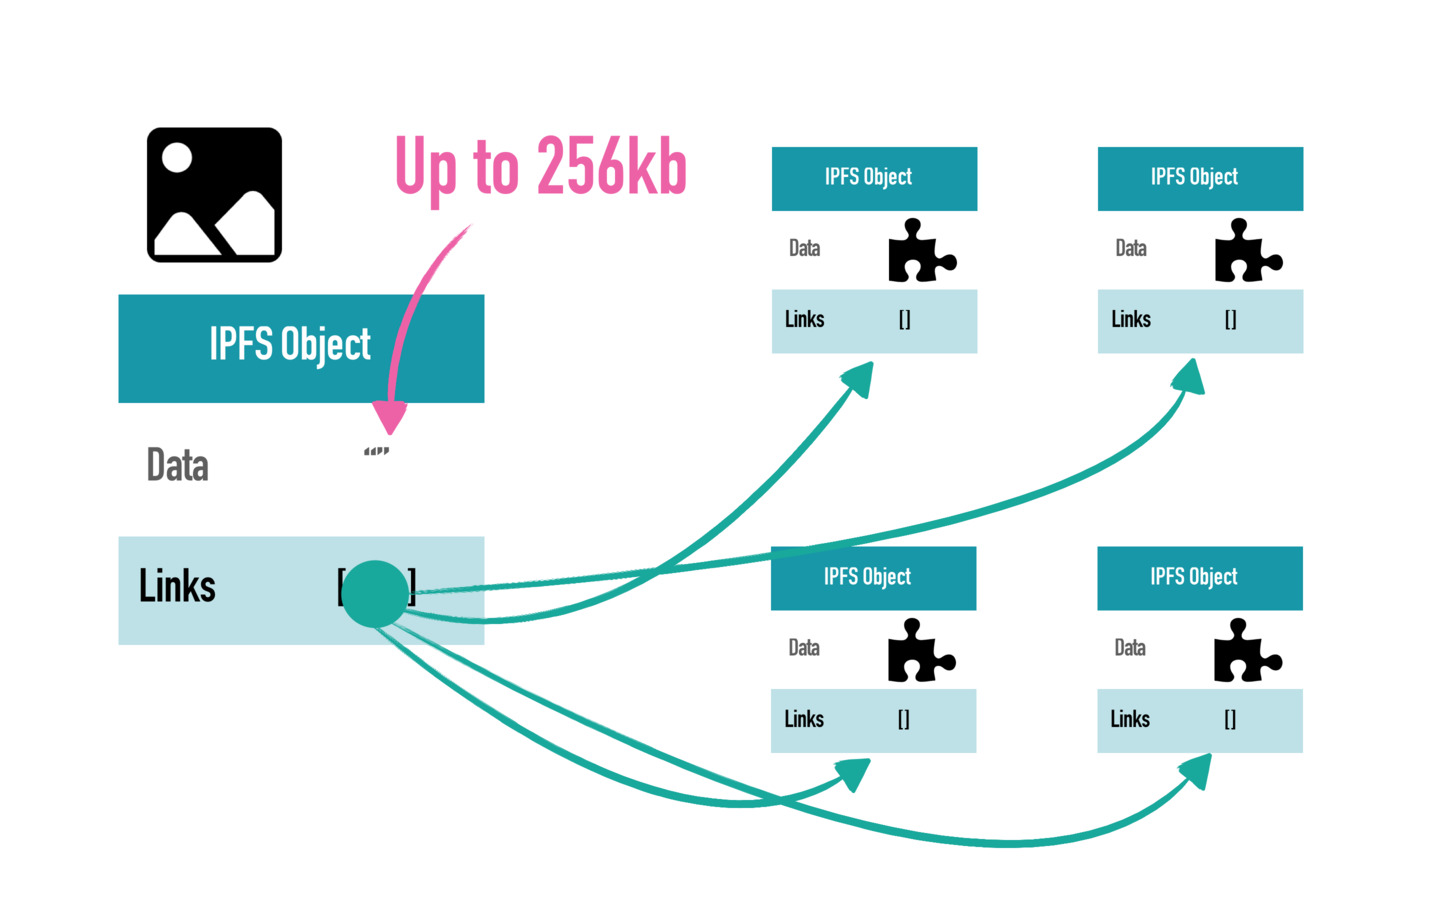
\includegraphics[width=15cm]{img/IPFSExample.png}
    \caption{A file being stored in the \ac{IPFS} network}
    \label{fig:IPFSExample}
\end{figure}


The properties of this \ac{DFS} provide meaningful advantages to work with Blockchain Systems since both work decentralized, trustless and in a set of hashed blocks.